\documentclass{standalone}

\usepackage{tikz}
\usepackage{amsmath}
\usetikzlibrary{math}

% definition of all the colors
\usepackage{xcolor}
%
% genertated by ./compile.py
%

\definecolor{codegreen}{RGB}{0, 153, 0}
\definecolor{codegray}{RGB}{127, 127, 127}
\definecolor{codeblue}{RGB}{102, 214, 237}
\definecolor{codekeyword}{RGB}{249, 36, 114}
\definecolor{codecomment}{RGB}{127, 127, 127}
\definecolor{backcolor}{RGB}{242, 242, 235}
\definecolor{linkcolor}{RGB}{102, 0, 0}
\definecolor{corange}{RGB}{255, 70, 0}
\definecolor{cyellow}{RGB}{209, 153, 0}
\definecolor{cblue}{RGB}{64, 128, 255}
\definecolor{cbrown}{RGB}{153, 102, 51}
\definecolor{cpink}{RGB}{255, 0, 255}
\definecolor{cred}{RGB}{255, 64, 0}
\definecolor{cgreen}{RGB}{0, 191, 0}
\definecolor{clightblue}{RGB}{191, 217, 255}
\definecolor{cturquois}{RGB}{0, 255, 255}
\definecolor{cpurple}{RGB}{128, 0, 255}
\definecolor{clightgreen}{RGB}{175, 255, 175}
\definecolor{clightpink}{RGB}{255, 175, 255}
\definecolor{cdarkblue}{RGB}{0, 0, 255}
\definecolor{cdarkred}{RGB}{255, 0, 0}
\definecolor{cdarkgreen}{RGB}{0, 255, 0}


\begin{document}

%\tikzset{every picture/.style={line width=0.75pt}} %set default line width to 0.75pt        

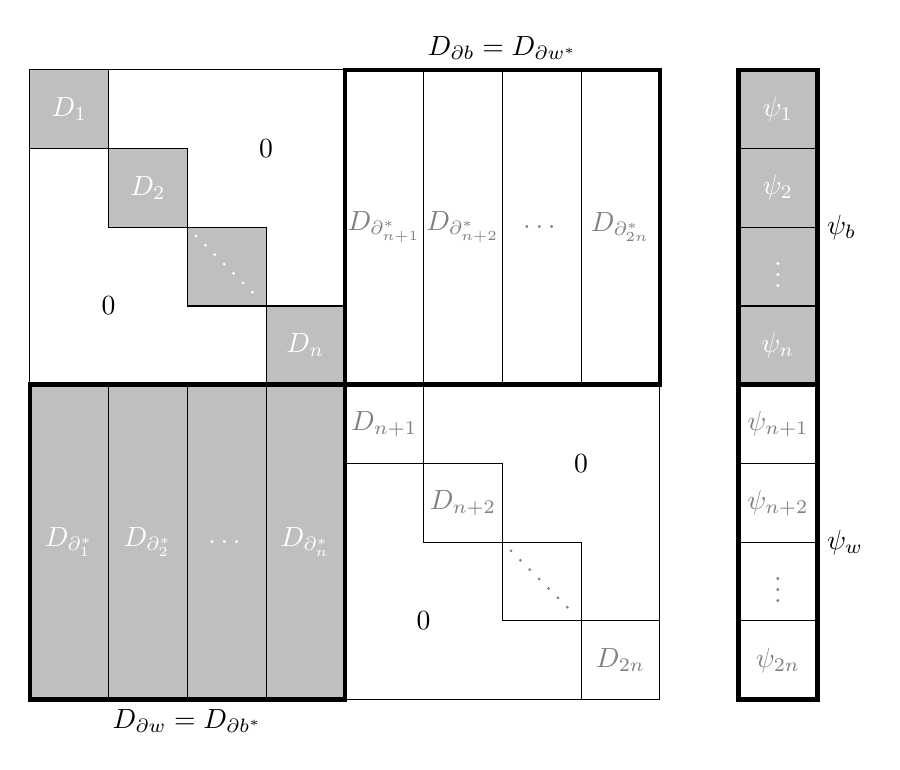
\begin{tikzpicture}[]

\def\step{1}
\def\eps{0.1}

% matrix
\draw[black, thin] (0,0) rectangle (8,8); % full rectangle of the matrix

\draw[draw=none]                   (\step*2,\step*6) rectangle (\step*4,\step*8)  node[pos=.5] {\textcolor{black}{$0$}};
\draw[draw=none]                   (\step*0,\step*4) rectangle (\step*2,\step*6)  node[pos=.5] {\textcolor{black}{$0$}};
\draw[black, thin, fill=lightgray] (\step*0,\step*7) rectangle (\step*1,\step*8)  node[pos=.5] {\textcolor{white}{$D_1$}};
\draw[black, thin, fill=lightgray] (\step*1,\step*6) rectangle (\step*2,\step*7)  node[pos=.5] {\textcolor{white}{$D_2$}};
\draw[black, thin, fill=lightgray] (\step*2,\step*5) rectangle (\step*3,\step*6);
\pgfmathsetmacro\xs{(2 + \eps)*\step}
\pgfmathsetmacro\xe{(3 - \eps)*\step}
\pgfmathsetmacro\ys{(6 - \eps)*\step}
\pgfmathsetmacro\ye{(5 + \eps)*\step}
\draw[white, thick, loosely dotted] (\xs,\ys) -- (\xe,\ye);
\draw[black, thin, fill=lightgray] (\step*3,\step*4) rectangle (\step*4,\step*5)  node[pos=.5] {\textcolor{white}{$D_n$}};

\draw[draw=none]                   (\step*4,\step*0) rectangle (\step*6,\step*2)  node[pos=.5] {\textcolor{black}{$0$}};
\draw[draw=none]                   (\step*6,\step*2) rectangle (\step*8,\step*4)  node[pos=.5] {\textcolor{black}{$0$}};
\draw[black, thin, fill=white] (\step*4,\step*3) rectangle (\step*5,\step*4)  node[pos=.5] {\textcolor{gray}{$D_{n+1}$}};
\draw[black, thin, fill=white] (\step*5,\step*2) rectangle (\step*6,\step*3)  node[pos=.5] {\textcolor{gray}{$D_{n+2}$}};
\draw[black, thin, fill=white] (\step*6,\step*1) rectangle (\step*7,\step*2);
\pgfmathsetmacro\xs{(6 + \eps)*\step}
\pgfmathsetmacro\xe{(7 - \eps)*\step}
\pgfmathsetmacro\ys{(2 - \eps)*\step}
\pgfmathsetmacro\ye{(1 + \eps)*\step}
\draw[gray, thick, loosely dotted] (\xs,\ys) -- (\xe,\ye);
\draw[black, thin, fill=white] (\step*7,\step*0) rectangle (\step*8,\step*1)  node[pos=.5] {\textcolor{gray}{$D_{2n}$}};

% boundary operator for every white block
\draw[black, thin]                 (\step*4,\step*4) rectangle (\step*5,\step*8)   node[pos=.5] {\textcolor{gray}{$D_{\partial_{n+1}^{*}}$}};
\draw[black, thin]                 (\step*5,\step*4) rectangle (\step*6,\step*8)   node[pos=.5] {\textcolor{gray}{$D_{\partial_{n+2}^{*}}$}};
\draw[black, thin]                 (\step*6,\step*4) rectangle (\step*7,\step*8)   node[pos=.5] {\textcolor{gray}{$\dots$}};
\draw[black, thin]                 (\step*7,\step*4) rectangle (\step*8,\step*8)   node[pos=.5] {\textcolor{gray}{$D_{\partial_{2n}^{*}}$}};

% boundary operator for every black block
\draw[black, thin, fill=lightgray] (\step*0,\step*0) rectangle (\step*1,\step*4)   node[pos=.5] {\textcolor{white}{$D_{\partial_{1}^{*}}$}};
\draw[black, thin, fill=lightgray] (\step*1,\step*0) rectangle (\step*2,\step*4)   node[pos=.5] {\textcolor{white}{$D_{\partial_{2}^{*}}$}};
\draw[black, thin, fill=lightgray] (\step*2,\step*0) rectangle (\step*3,\step*4)   node[pos=.5] {\textcolor{white}{$\dots$}};
\draw[black, thin, fill=lightgray] (\step*3,\step*0) rectangle (\step*4,\step*4)   node[pos=.5] {\textcolor{white}{$D_{\partial_{n}^{*}}$}};

% white boundary operator
%\draw[black, thick]                (\step*4,\step*4) rectangle (\step*8,\step*8)   node[pos=.5] {\textcolor{gray}{$D_{\partial b} = D_{\partial w^{*}}$}};
\draw[black, ultra thick]          (\step*4,\step*4) rectangle (\step*8,\step*8);
\node[above] at (\step*6,\step*8){$D_{\partial b} = D_{\partial w^{*}}$};

% black boundary operator
%\draw[black, thin, fill=lightgray] (0,0)             rectangle (\step*4,\step*4)   node[pos=.5] {\textcolor{white}{$D_{\partial w} = D_{\partial b^{*}}$}};
\draw[black, ultra thick]          (\step*0,\step*0) rectangle (\step*4,\step*4);
\node[below] at (\step*2,\step*0){$D_{\partial w} = D_{\partial b^{*}}$};


% vector
\draw[black, thin] (9,0) rectangle (10,8); % full rectangle of the vector

\draw[black, thin, fill=lightgray] (\step*9,\step*7) rectangle (\step*10,\step*8)  node[pos=.5] {\textcolor{white}{$\psi_1$}};
\draw[black, thin, fill=lightgray] (\step*9,\step*6) rectangle (\step*10,\step*7)  node[pos=.5] {\textcolor{white}{$\psi_2$}};
\draw[black, thin, fill=lightgray] (\step*9,\step*5) rectangle (\step*10,\step*6)  node[pos=.5] {\textcolor{white}{$\vdots$}};
\draw[black, thin, fill=lightgray] (\step*9,\step*4) rectangle (\step*10,\step*5)  node[pos=.5] {\textcolor{white}{$\psi_n$}};

\draw[black, thin, fill=white]     (\step*9,\step*3) rectangle (\step*10,\step*4)  node[pos=.5] {\textcolor{gray}{$\psi_{n+1}$}};
\draw[black, thin, fill=white]     (\step*9,\step*2) rectangle (\step*10,\step*3)  node[pos=.5] {\textcolor{gray}{$\psi_{n+2}$}};
\draw[black, thin, fill=white]     (\step*9,\step*1) rectangle (\step*10,\step*2)  node[pos=.5] {\textcolor{gray}{$\vdots$}};
\draw[black, thin, fill=white]     (\step*9,\step*0) rectangle (\step*10,\step*1)  node[pos=.5] {\textcolor{gray}{$\psi_{2n}$}};

\draw[black, ultra thick]          (\step*9,\step*4) rectangle (\step*10,\step*8);
\node[right] at (\step*10,\step*6){$\psi_b$};

\draw[black, ultra thick]          (\step*9,\step*0) rectangle (\step*10,\step*4);
\node[right] at (\step*10,\step*2){$\psi_w$};

\end{tikzpicture}


\end{document}